\documentclass[margin=0px]{article}

\usepackage{listings}
\usepackage[utf8]{inputenc}
\usepackage{graphicx}
\usepackage{float}
\usepackage[a4paper, margin=1in]{geometry}
\usepackage{amsthm}
\usepackage{amssymb}

\makeatletter
\renewcommand\paragraph{%
	\@startsection{paragraph}{4}{0mm}%
	{-\baselineskip}%
	{.5\baselineskip}%
	{\normalfont\normalsize\bfseries}}
\makeatother

\renewcommand{\figurename}{ábra}
\newenvironment{tetel}[1]{\paragraph{#1}}{}
% A dokument itt kezdődik

\title{Záróvizsga tételsor \\ \large 19. Adatbázisok optimalizálása és konkurencia kezelése}
\date{}
\author{Ancsin Ádám}

\begin{document}

	\maketitle
	
	\begin{tetel}{Adatbázisok optimalizálása és konkurencia kezelése}
			Az adatbázis-kezelő rendszerek feladata, részei. Indexstruktúrák, lekérdezések végrehajtása, optimalizálási stratégiák. Tranzakciók feldolgozása, naplózás és helyreállítás, konkurencia-kezelés.
	\end{tetel}
	
	
	\section{Az adatbázis-kezelő rendszerek feladata, részei}
	
	Adatbázis-kezelő rendszer alatt olyan számítógépprogramot értünk, mely megvalósítja nagy tömegű adat biztonságos
	tárolását, gyors lekérdezhetőségét és módosíthatóságát, tipikusan egyszerre	több felhasználó számára.
	
	Az adatbázis-kezelési tevékenységeket két csoportra szokás osztani: adatmanipulációra (lekérdezés),
	illetve definiálásra (adatszerkezetek kialakítása, módosítása). Az adatok manipulációjára szolgáló nyelveket összefoglalóan
	Data Manipulation Language-nek (DML), míg a definíciós eszközökkel rendelkező nyelveket Data Definition Language-nek (DDL)
	szokás nevezni.
	
	\begin{figure}[H]
		\centering
		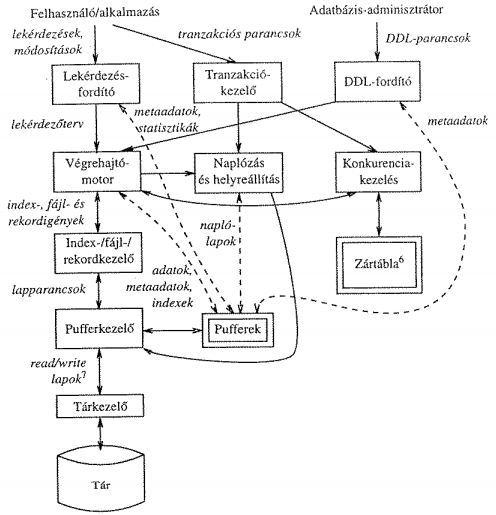
\includegraphics[width=0.7\linewidth]{img/db_felepites}
		\caption{Az adatbázis-kezelő rendszer alkotórészei.}
		\label{fig:db_felepites}
	\end{figure}
	
	\subsection{Az egyes alkotórészek rövid jellemzése}
	\noindent \textbf{Lekérdezésfordító}: A lekérdezésfordító elemzi és optimalizálja a lekérdezést, ami alapján
	elkészíti a lekérdezés-végrehajtási tervet (lekérdezéstervet).\\
	
	\noindent \textbf{Végrehajtómotor}: A végrehajtómotor a lekérdezésfordítótól megkapja a lekérdezéstervet, majd kisebb
	adatdarabokra (tipikusan rekordokra, egy reláció soraira) vonatkozó kérések sorozatát adja át az erőforrás-kezelőnek.\\
	
	\noindent \textbf{Erőforrás-kezelő}: Az erőforrás-kezelő ismeri a relációkat tartalmazó adatfájlokat, a fájlok
	rekordjainak formátumát, méretét, valamint az indexfájlokat. Az adatkéréseket az erőforrás-kezelő lefordítja lapokra,
	amit átad a pufferkezelőnek.\\
	
	\noindent \textbf{Pufferkezelő}: Feladata, hogy a másodlagos adattárolóról (lemez, stb.) az adatok megfelelő részét olvassa
	be a központi memória puffereibe. A pufferkezelő információkat cserél a tárkezelővel, hogy megkapja az adatokat
	a lemezről.\\
	
	\noindent \textbf{Tárkezelő}: Adatokat ír-olvas a másodlagos adattárolóról. Előfordulhat, hogy igénybe veszi az oprendszer
	parancsait is, de sokszor közvetlenül a lemezkezelőhöz intézi a parancsait.\\
	
	\noindent \textbf{Tranzakciókezelő}: A lekérdezéseket és más tevékenységeket tranzakciókba szervezzük. A tranzakciók olyan
	egységek, amelyeket atomosan és elkülöníthetően kell végrehajtani, valamint a végrehajtásnak tartósnak kell lennie, illetve
	a tranzakció végrehajtása nem állíthat elő érvénytelen adatbázis-állapotot (azaz konzisztens). Ezeket a követelményeket
	az ACID mozaikszóval szokás összefoglalni. A tranzakciókezelő hajtatja végre a tranzakciókat és gondoskodik a naplózásról
	és helyreállításról, valamint a konkurenciakezelésről.\\
	
	\section{Indexstruktúrák}
	
	Az indexek keresést gyorsító segédstruktúrák. Több mezőre is lehet indexet készíteni. Nem csak a
	főfájlt, hanem az indexet is karban kell tartani, ami plusz költséget jelent. Ha a keresési mező egyik
	indexmezővel sem esik egybe akkor kupac szervezést jelent. Az indexrekordok szerkezete (a,p) , ahol
	"a" egy  érték  az  indexelt  oszlopban, "p" egy  blokkmutató, arra a  blokkra mutat, amelyben az A=a
	értékű rekordot tároljuk. Az index mindig rendezett az indexértékek szerint.
	
	\subsection{Elsődleges index}
	
	Elsődleges index esetén a főfájl  is  rendezett  (az  indexmező  szerint), így emiatt csak egy elsődleges 
	indexet lehet megadni.  Elég  a  főfájl  minden  blokkjának  legkisebb  rekordjához  készíteni 
	indexrekordot, így azok száma: $T(I)  = B$ (ritka index). Indexrekordból sokkal több fér egy blokkba, mint 
	a  főfájl  rekordjaiból:  $bf(I)  >> bf$,  azaz  az  indexfájl  sokkal  kisebb  rendezett  fájl,  mint  a  főfájl:
	$B(I) = \frac{B}{bf(I)} << B = \frac{T}{bf}$. 
	
	Keresésnél, mivel az indexfájlban nem szerepel minden érték, ezért csak fedő értéket kereshetünk, a 
	legnagyobb olyan indexértéket, amely a keresett értéknél kisebb vagy egyenlő. Fedő érték keresése 
	az index rendezettsége miatt bináris kereséssel történik: $\log_{2}(B(I))$. A fedő indexrekordban szereplő 
	blokkmutatónak megfelelő blokkot még be kell olvasni. Így a költség $1+\log_{2}(B(I)) << \log_{2}(B)$(rendezett 
	eset).
	Módosításnál a rendezett fájlba kell beszúrni. Ha az első rekord változik a blokkban, akkor az 
	indexfájlba is be kell szúrni, ami szintén rendezett. A megoldás az, hogy üres helyeket hagyunk a 
	főfájl, és az indexfájl blokkjaiban is. Ezzel a tárméret duplázódhat, de a beszúrás legfeljebb egy 
	főrekord, és egy indexrekord visszaírását jelenti.
	
	\subsection{Másodlagos index}
	
	Másodlagos index esetén a főfájl rendezetlen (az indexfájl mindig rendezett). Másodlagos indexből 
	többet is meg lehet adni. A főfájl minden rekordjához kell készíteni indexrekordot, így az 
	indexrekordok száma: $T(I) = T$ (sűrű index). Indexrekordból sokkal több fér egy blokkba, mint a főfájl 
	rekordjaiból: $bf(I) >> bf$, azaz az indexfájl sokkal kisebb fájl, mint a főfájl: $B(I) = \frac{T}{bf(I)} << 
	B=\frac{T}{bf}$.
	Az indexben a keresés az index rendezettsége miatt bináris kereséssel történik: $\log_{2}(B(I))$ . A talált 
	indexrekordban szereplő blokkmutatónak megfelelő blokkot még be kell olvasni. Így a költség
	$1+\log_{2}(B(I)) << \log_{2}(B)$ (rendezett eset). Az elsődleges indexnél rosszabb a keresési idő, mert több az 
	indexrekord.
	A főfájl kupac szervezésű. Rendezett fájlba kell beszúrni. Ha az első rekord változik a blokkban, akkor 
	az indexfájlba is be kell szúrni, ami szintén rendezett. Megoldás: üres helyeket hagyunk a főfájl, és az 
	indexfájl blokkjaiban is. Ezzel a tárméret duplázódhat, de a beszúrás legfeljebb egy főrekord és egy 
	indexrekord visszaírását jelenti.
	
	\subsection{Bitmap index}
	
	A bitmap indexeket az oszlopok adott értékeihez szokták hozzárendelni, az alábbi módon:
	\begin{itemize}
		\item	Ha az oszlopban az $i$. sor értéke megegyezik az adott értékkel, akkor a bitmap index $i$. tagja 
		egy 1-es.	
		
		\item	Ha az oszlopban az $i$. sor értéke viszont nem egyezik meg az adott értékkel, akkor a bitmap 
		index $i$. tagja egy 0.
	\end{itemize}

	Így egy lekérdezésnél csak megfelelően össze kell AND-elni, illetve OR-olni a bitmap indexeket, és az 
	így kapott számsorozatban megkeresni, hol van 1-es.
	A bináris értékeket szokás szakaszhossz kódolással tömöríteni a hatékonyabb tárolás érdekében.
		
	\subsection{Többszintű indexek}
	
	Az indexfájl (1. indexszint) is fájl, ráadásul rendezett, így ezt is meg lehet indexelni, elsődleges index-
	szel. A főfájl lehet rendezett vagy rendezetlen (az indexfájl mindig rendezett) . A $t$. szintű index: az 
	indexszinteket is indexeljük, összesen $t$ szintig.
	A $t$. szinten ($I(t)$)  bináris kereséssel keressük meg a fedő indexrekordot. Követjük a mutatót, minden 
	szinten, és végül a főfájlban: $\log_{2}(B(I(t))) + t$ blokkolvasás. Ha a legfelső szint 1 blokkból áll, akkor $t+1$
	blokkolvasást jelent. Minden szint blokkolási faktora megegyezik, mert egyforma hosszúak az 
	indexrekordok.
	
	A $t$. szinten 1 blokk: $1=\frac{B}{bf(I)^{t}}$. Azaz $t=\log_{bf(I)}(B) < \log_{2}(B) $, tehát jobb a rendezett fájlszervezésnél. A 
	$log_{bf(I)}(B) < \log_{2}(B(I)) $ is teljesül általában, így az egyszintű indexeknél is
	gyorsabb.
	
	\subsection{B-fa index}
	
	Logikailag az index egy rendezett lista. Fizikailag a rendezett sorrendet táblába rendezett mutatók 
	biztosítják. A fa struktúrájú indexek B-fákkal ábrázolhatóak. A B-fák megoldják a bináris fák 
	kiegyenlítetlenségi problémáját, mivel "alulról" töltjük fel őket. A B-fa egy csomópontjához több 
	kulcsérték tartozhat. A mutatók más csomópontokra mutatnak, és így az összes kulcsértékre az adott 
	csomóponton.
	
	Mivel a B-fák kiegyenlítettek (minden ág egyenlő hosszú, vagyis ugyanazon a szinten fejeződik be), 
	kiküszöbölik a változó elérési időket, amik a bináris fákban megfigyelhetőek. Bár a kulcsértékek és a 
	hozzájuk kapcsolódó címek még mindig a fa minden szintjén megtalálhatók, és ennek eredménye:
	egyenlőtlen elérési utak, és egyenlőtlen elérési idő, valamint komplex fakeresési algoritmus az 
	adatfájl logikailag soros olvasására. Ez kiküszöbölhető, ha nem engedjük meg az adatfájl címek 
	tárolását levélszint felett. Ebből következően: minden elérés ugyanolyan hosszú utat vesz igénybe, 
	aminek egyenlő elérési idő az eredménye, és egy logikailag soros olvasása az adatfájlnak a levélszint 
	elérésével megoldható. Nincs szükség komplex fakeresési algoritmusra.
	
	A $B^{+}$-fa egy olyan B-fa, mely legalább 50\%-ban telített. A szerkezeten kívül a telítettséget biztosító 
	karbantartó algoritmusokat is beleértjük.
	
	A $B^{*}$-fa egy olyan B-fa, mely legalább 66\%-ban telített.
	
	\subsection{Hasító index}
	
	A rekordok edényekbe (bucket) particionálva helyezkednek el, melyekre a $h$ hasítómezőn értelmezett
	függvény osztja szét őket. Hatékony egyenlőségi keresés, beszúrás, és törlés jellemzi, viszont nem támogatja
	az intervallumos keresést. 
	
	A rekordokat blokkláncokba soroljuk, és a blokklánc utolsó blokkjának
	első üres helyére tesszük a rekordokat a beérkezés sorrendjében. A blokkláncok száma lehet előre adott
	(statikus hasítás, ekkor a számot K-val jelöljük), vagy a tárolt adatok alapján változhat (dinamikus hasítás).
	A besorolás az indexmező értékei alapján történik. Egy $h(x) \in \left\{1,..,K\right\}$ hasító függvény értéke mondja meg,
	hogy melyik kosárba tartozik a rekord, ha $x$ volt az indexmező értéke a rekordban. A hasító függvény
	általában maradékos osztáson alapul (például $mod(K)$). Akkor jó egy hasító függvény, ha nagyjából egyforma
	hosszú blokkláncok keletkeznek, azaz egyenletesen sorolja be a rekordokat. Ekkor a blokklánc $\frac{B}{K}$ blokkból áll.\\
	
	\noindent A keresés költsége:
	\begin{itemize}
		\item	Ha az indexmező és keresési mező eltér, akkor kupac szervezést jelent.
		\item	Ha az indexmező és keresési mező megegyezik, akkor csak elég a $h(a)$ sorszámú kosarat végignézni,
		amely $\frac{B}{K}$blokkból álló kupacnak felel meg, azaz $\frac{B}{K}$ legrosszabb esetben.
		A keresés így $K$-szorosára gyorsul.
	\end{itemize}
	
	A tárméret $B$, ha minden blokk nagyjából tele van. Nagy $K$ esetén azonban sok olyan blokklánc lehet,
	amely egy blokkból fog állni, és a blokkban is csak 1 rekord lesz. Ekkor a keresési idő: 1 blokkbeolvasás,
	de $B$ helyett $T$ számú blokkban tároljuk az adatokat. Módosításnál $\frac{B}{K}$ blokkból álló kupac
	szervezésű kosarat kell módosítani.
	
	\section{Lekérdezések végrehajtása, optimalizálása}
	
	A lekérdezésfeldolgozó egy relációs adatbázis-kezelő komponenseinek azon csoportja, amelyik a felhasználó lekérdezéseit,
	valamint adatmódosító utasításait lefordítja adatbázis-műveletekre, amiket végre is hajt.
	
	\begin{figure}[H]
		\centering
		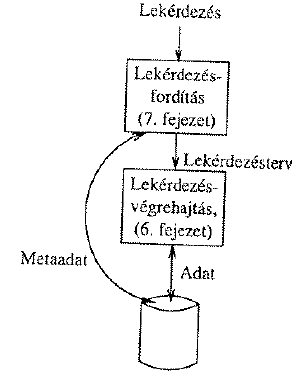
\includegraphics[width=0.3\linewidth]{img/queryprocessing}
		\caption{A lekérdezésfeldolgozás lépései.}
		\label{fig:queryprocessing}
	\end{figure}
	
	A lekérdezés végrehajtása tulajdonképpen az adatbázist manipuláló algoritmusok összessége, azonban a végrehajtás
	előtt szükség van a lekérdezések fordítására. \\
	
	\noindent A lekérdezés-fordítás lépései:
	\begin{enumerate}
		\item	Elemzés: egy elemző fát építünk fel, amely a lekérdezést és annak szerkezetét jellemzi
		
		\item	Lekérdezésátírás: Az elemző fából egy kezdeti lekérdezéstervet készítünk, amelyet átalakítunk
		egy ezzel ekvivalens tervvé, aminek végrehajtási ideje várhatóan kisebb lesz. Elkészül a logikai
		lekérdezésterv, amely relációs algebrai kifejezéseket tartalmaz.
		
		\item	A logikai tervet átalakítjuk fizikai tervvé úgy, hogy a logikai terv operátoraihoz kiválasztunk egy
		algoritmust,  valamint meghatározzuk az operátorok végrehajtási sorrendjét. A fizikai terv olyan részleteket is
		tartalmaz, hogy pl. kell-e rendezni, hogyan férünk hozzá az adatokhoz.
	\end{enumerate}
	
	\begin{figure}[H]
		\centering
		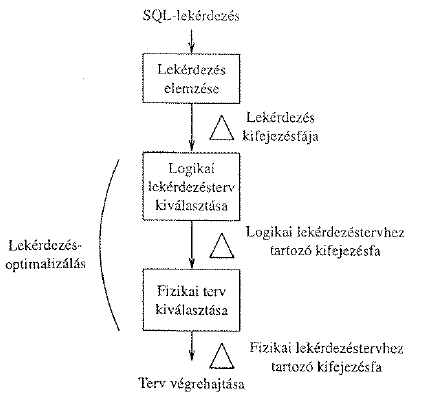
\includegraphics[width=0.5\linewidth]{img/querycompiling}
		\caption{A lekérdezésfordítás lépései.}
		\label{fig:querycompiling}
	\end{figure}
	
	\subsection{Algebrai optimalizálás}
	
	A relációs algebrai kifejezéseket minél gyorsabban akarjuk kiszámolni. A kiszámítás költsége arányos a relációs algebrai kifejezés részkifejezéseinek megfelelő relációk tárolási méreteinek összegével. A módszer az, hogy műveleti tulajdonságokon alapuló ekvivalens átalakításokat alkalmazunk, azért, hogy várhatóan kisebb méretű relációk keletkezzenek. Az eljárás heurisztikus, tehát nem az argumentum relációk valódi méretével számol. Az eredmény nem egyértelmű, ugyanis az átalakítások sorrendje nem determinisztikus, így más sorrendben végrehajtva az átalakításokat más végeredményt kaphatunk, de mindegyik általában jobb költségű, mint amiből kiindultunk.\\
	
	\noindent Az optimalizáló algoritmus a következő heurisztikus elveken alapul:
	\begin{itemize}
		\item	Minél hamarabb szelektáljunk, hogy a részkifejezések várhatóan kisebb relációk legyenek. 
		\item	A szorzás utáni kiválasztásokból próbáljunk természetes összekapcsolásokat képezni, mert az összekapcsolás hatékonyabban kiszámolható, mint a szorzatból történő kiválasztás.
		\item	Vonjuk össze az egymás utáni unáris műveleteket (kiválasztásokat és vetítéseket), és ezekből lehetőleg egy kiválasztást, vagy vetítést, vagy kiválasztás utáni vetítést képezzünk. Így csökken a műveletek száma, és általában a kiválasztás kisebb relációt eredményez, mint a vetítés.
		\item	Keressünk közös részkifejezéseket, amiket így elég csak egyszer kiszámolni a kifejezés kiértékelése során.
	\end{itemize}
	
	\subsection{Relációs algebrai műveletek megvalósítása}
	
	\subsubsection{Kiválasztás}
	
	A kiválasztás ($\sigma$) lehetséges megvalósításai:
	\begin{itemize}
		\item	Lineáris keresés: Olvassunk be minden lapot és keressük az egyezéseket (egyenlőségvizsgálat esetén).
		Az átlagos költség a lapok száma, ha a mező nem kulcs, illetve a lapok számának fele, ha a mező kulcs.
		\item	Bináris (logaritmikus) keresés: Csak rendezett mező esetén használható.
		\item	Elsődleges index használata.
		\item	Másodlagos index használata.
	\end{itemize}
	
	\noindent \textbf{Összetett kiválasztás}: Előfordulhat, hogy több feltétel van, amelyek és/vagy kapcsolatban vannak egymással.
	Megvalósítása:
	\begin{itemize}
		\item	Konjunkciós kiválasztás esetén ($\sigma_{\theta_{1} \wedge ... \wedge \theta_{n}}$): 
		\begin{itemize}
			\item	Válasszuk ki a legkisebb költségű $\sigma_{\theta_{i}}$-t, és azt végezzük el (lásd fent),
			majd az eredményt szűrjük a többi feltételre. A költség az egyszerű kiválasztás költsége lesz a kiválasztott $\sigma_{\theta_{i}}$-re.
			
			\item	Ha mindegyik $\theta_{i}$ mezőjére van indexünk, akkor keressük az indexekben és adjuk vissza a megfelelő
			sorok rowid-jeit. Végül vegyük ezek metszetét. A költség az indexekben való keresés összköltsége + a rekordok beolvasása.
		\end{itemize}
		
		\item	Diszjunkciós kiválasztás esetén ($\sigma_{\theta_{1} \vee ... \vee \theta_{n}}$):
		\begin{itemize}
			\item	Lineáris keresés.
				
			\item	Ha mindegyik $\theta_{i}$ mezőjére van indexünk, akkor keressük az indexekben és adjuk vissza a megfelelő
			sorok rowid-jeit. Végül vegyük ezek unióját. A költség az indexekben való keresés összköltsége + a rekordok beolvasása.
			\end{itemize}
	\end{itemize}
	
	\subsubsection{Vetítés és halmazműveletek}
	
	Vetítésnél és halmazműveleteknél a duplikátumokat ki kell szűrni.\\
	
	\noindent \textbf{Vetítés ($\pi$) megvalósítása}:
	
	\begin{enumerate}
		\item	Kezdeti átnézés: eldobjuk a felesleges mezőket.
		\item	Duplikátumok törlése: ehhez az eredményt rendezzük az összes mező szerint, így a duplikáltak szomszédosak
		lesznek. Ezeket kell eldobni.
	\end{enumerate}
	
	\noindent A költség a kezdeti átnézés, a rendezés és a duplikátumok törlésének összköltsége lesz.
	
	\subsubsection{Összekapcsolások}
	
	Az összekapcsolásokat (join) többféle módon is el lehet végezni:
	
	\begin{itemize}
		\item	\textbf{Beágyazott ciklusú összekapcsolás (nested loop join)}: Bármekkora méretű relációra használható, nem szükséges, hogy
		az egyik reláció elférjen a memóriában. Két fajtája van, a sor és a blokk alapú.
		\begin{itemize}
			\item	\textbf{Sor alapú beágyazott ciklusú összekapcsolás}: Legyen R és S a két összekapcsolandó reláció, ezek közül jelölje
			S a kisebb méretűt, ez lesz a belső reláció, R pedig a külső. Az algoritmus a következő: menjünk végig R (a külső reláció)
			összes során és R minden egyes soránál menjünk végig a belső reláció, S összes során. Ha az aktuálisan vizsgált 2 sor összekapcsolható, akkor írjuk bele az eredménybe. Jó esetben S belefér a memóriába, ekkor csak egyszer kell beolvasni S-t,
			majd mindvégig a memóriában tarthatjuk. Ebben az esetben mindkét reláció lapjait egyszer kell beolvasni. Legrosszabb
			esetben mindkét relációból csak egy-egy lap fér bele a memóriába. Ekkor R minden egyes soránál végig kell olvasni S-t.
			
			\item	\textbf{Blokk alapú beágyazott ciklusú összekapcsolás}: Az előbbihez képest annyi a különbség, hogy nem soronként
			megyünk végig a relációkon. Legyen M a memóriába férő lapok száma. Ekkor minden egyes iterációban R-nek M-1 lapját olvassuk
			be, majd szervezzük ezeket valamilyen keresési struktúrába, ahol a kulcs az R és S közös attribútumai. Ezután menjünk
			végig laponként S-en, és S memóriában lévő soraiból keressük meg azokat, amelyek összekapcsolhatóak valamely R-ből
			beolvasott sorral, majd írjuk bele ezeket az eredményrelációba.
		\end{itemize}
		
		\item	\textbf{Összefésüléses rendező összekapcsolás (merge join)}: A relációk az összekapcsolási mezők szerint rendezettek.
		Egyesítjük a rendezett relációkat: mutatók az első rekordra mindkét relációban. Beolvasunk S-ből egy rekordcsoportot, ahol az összekapcsolási attribútum értéke megegyezik. Beolvasunk rekordokat R-ből és feldolgozzuk. A rendezett relációkat
		csak egyszer kell végigolvasni, ezért az összekapcsolás költsége: rendezés költsége + a 2 reláció lapjainak száma.
		
		\item	\textbf{Hasításos összekapcsolás (hash join)}: Az összekapcsolási attribútumot használjunk hasítókulcsként, ez alapján
		particionáljuk R és S sorait hasítással. Ha mindegyik táblából $n$ kosarat szeretnénk, akkor az eredmény: $R_{0},R_{1},..R_{n-1}, S_{0},S_{1},..,S_{n-1}$ kosarak. Ezután az egymáshoz rendelt kosárpárokat összekapcsoljuk blokk alapú beágyazott ciklusú
		összekapcsolással, hasítófüggvény alapú indexet használva.
	\end{itemize}
	
	\noindent \textbf{Több tábla összekapcsolása}: Az összekapcsolások kommutatívak és asszociatívak, ezért az eredmény szempontjából
	mindegy, hogy milyen sorrendben kapcsoljuk őket össze. A sorrend viszont befolyásolhatja a hatékonyságot, ugyanis rossz választás
	esetén a köztes eredmények nagy méretűek lesznek.\\
	
	\noindent A legjobb összekapcsolási fa megtalálása $n$ reláció egy halmazához:
	\begin{itemize}
		\item	Hogy megtaláljuk a legjobb összekapcsolási fát n reláció egy $S$ halmazához,
		vegyük az összes lehetséges tervet mely így néz ki: $S_{1} \Join (S - S_{1})$, ahol $S_{1}$ az $S$ tetszőleges nem üres részhalmaza.
		
		\item	Rekurzívan számítsuk ki $S$ részhalmazainak összekapcsolásának költségeit, hogy meghatározzuk minden egyes terv költségét. Válasszuk a legolcsóbbat.
		
		\item	Mikor bármely részhalmaz terve kiszámításra került, az újbóli kiszámítás helyett tároljuk el és hasznosítsuk újra amikor ismét szükség lesz rá.
	\end{itemize}
	
	\section{Tranzakciókezelés}
	
	\noindent \textbf{Konzisztens adatbázis}: Az adatbázisokra különböző megszorítások adhatóak meg. Az adatbázis konzisztens állapotban
	van, ha kielégíti az összes ilyen megszorítást. Konzisztens adatbázis egy olyan adatbázis, amely konzisztens állapotban van.\\
	
	\noindent A konzisztencia sérülhet a következő esetekben:
	\begin{itemize}
		\item	Tranzakcióhiba: hibásan megírt, rosszul ütemezett, félbehagyott tranzakciók.
		\item	Adatbázis--kezelési hiba: az adatbázis-kezelő valamelyik komponense nem, vagy rosszul hajtja végre a feladatát.
		\item	Hardverhiba: elvész egy adat, vagy megváltozik az értéke.
		\item	Adatmegosztásból származó hiba.
	\end{itemize}
	
	\noindent \textbf{Tranzakció}: Konzisztenciát tartó adatbázis-műveletek sorozata. Ezek után mindig feltesszük, hogy ha
	a T tranzakció indulásakor az adatbázis konzisztens állapotban van, akkor ha T egyedül fut le, az adatbázis konzisztens állapotban
	lesz a futás végén (közben kialakulhat inkonzisztens állapot).
	
	\noindent Helyesség feltétele:
	\begin{itemize}
		\item	Ha leáll egy vagy több tranzakció (abort, vagy hiba miatt), akkor is konzisztens adatbázist kapunk.
		\item	Minden egyes tranzakció induláskor konzisztens adatbázist lát.
	\end{itemize} 
	
	\noindent A tranzakcióktól a következő tulajdonságokat szoktuk elvárni (ACID):
	
	\begin{itemize}
		\item	Atomosság (A, azaz Atomicity): a tranzakció "mindent vagy semmit" jellegű végrehajtása (vagy teljesen végrehajtjuk, vagy egyáltalán nem hajtjuk végre).
		
		\item	Konzisztencia (C, azaz Consistency): az a feltétel, hogy a tranzakció megőrizze az adatbázis konzisztenciáját, azaz a tranzakció végrehajtása után is teljesüljenek az adatbázisban előírt konzisztenciamegszorítások. 
		
		\item	Elkülönítés (I, azaz Isolation): az a tény, hogy minden tranzakciónak látszólag úgy kell lefutnia, mintha ez alatt az idő alatt semmilyen másik tranzakciót sem hajtanánk végre.
		
		\item	Tartósság (D, azaz Durability): az a feltétel, hogy ha egyszer egy tranzakció befejeződött, akkor már soha többé nem veszhet el a tranzakciónak az adatbázison kifejtett hatása.	
	\end{itemize}
	A konzisztenciát mindig adottnak tekintjük. A másik három tulajdonságot viszont az adatbázis-kezelő rendszernek kell biztosítania, de ettől időnként eltekintünk. Feltesszük, hogy az adatbázis adategységekből, elemekből áll. Az adatbáziselem a fizikai adatbázisban tárolt adatok egyfajta funkcionális egysége, amelynek értékét tranzakciókkal lehet elérni (kiolvasni) vagy módosítani (kiírni). Adatbáziselem
	pl. a reláció, relációsor, lap.\\
	
	\subsection{A tranzakciók alaptevékenységei}
	
	\noindent A tranzakció és az adatbázis kölcsönhatásának 3 fontos helyszíne van:
	\begin{itemize}
		\item	Az adatbázis elemeit tartalmazó lemezblokkok területe.
		\item	A pufferkezelő által használt virtuális vagy valós memóriaterület.
		\item	A tranzakció memóriaterülete.
	\end{itemize}
	
	Ahhoz, hogy a tranzakció egy adatbáziselemet beolvashasson, azt előbb memóriapuffer(ek)be kell hozni, ha még nincs ott.
	Ezt követően tudja a puffer(ek) tartalmát a tranzakció saját memóriaterületére beolvasni. Az adatbáziselem új
	értékének kiírás fordítva történik: előbb a tranzakció kialakítja az új értéket saját memóriaterületén, majd ez
	az érték másolódik át a megfelelő puffer(ek)be.
	
	A pufferek tartalmának lemezre írásáról a pufferkezelő dönt. Vagy azonnal lemezre írja a változásokat, vagy nem.
	
	A naplózási algoritmusokn és más tranzakciókezelő algoritmusok tanulmányozása során különböző jelölésekre lesz szükség,
	melyekkel a különböző területek közötti adatmozgásokat írhatjuk le. A következő alapműveletek használjuk:
	
	\begin{itemize}
		\item	INPUT(X): Az X adatbáziselemet tartalmazó lemezblokk másolása a pufferbe.
		\item	READ(X,t): Az X adatbáziselem bemásolása a tranzakció $t$ lokális változójába. Ha az X-et tartalmazó blokk még
		nincs a memóriában, akkor INPUT(X)-et is beleértjük.
		\item	WRITE(X,t): A $t$ lokális változó tartalmaz az X adatbáziselem memóriapufferbeli tartalmába másolódik. Ha az X-et
		tartalmazó blokk még nincs a pufferben, akkor előbb INPUT(X) is végrehajtódik.
		\item	OUTPUT(X): Az X adatbáziselemet tartalmazó blokk kiírása lemezre.
	\end{itemize}

	\noindent A továbbiakban feltételezzük, hogy egy adatbáziselem nem nagyobb egy blokknál.
	
	\subsection{Naplózás és helyreállítás}
	
	Az adatokat meg kell védeni a rendszerhibáktól, ezért szükség van az adatok helyreállíthatóságára. Erre az elsődleges
	technika a naplózás, amely valamilyen biztonságos módszerrel rögzíti az adatbázisban végrehajtott módosítások történetét.
	
	A napló (log) nem más, mint naplóbejegyzések (log records) sorozata, melyek arról tartalmaznak információt, hogy mit tett
	egy tranzakció. Rendszerhiba esetén a napló segítségével rekonstruálható, hogy mit tett a tranzakció a hiba fellépéséig.
	
	\subsubsection{Naplóbejegyzések}
	
	Úgy kell tekintenünk, hogy a napló, mint fájl kizárólag bővítésre van megnyitva. Tranzakció végrehajtásakor a naplókezelőé
	a feladat, hogy minden fontos eseményt rögzítsen a naplóban.\\
	
	\noindent Az összes naplózási módszer által használt naplóbejegyzések:
	\begin{itemize}
		\item	$\langle START \ T \rangle$: Ez a bejegyzés jelzi a T tranzakció végrehajtásának kezdetét.
		\item	$\langle COMMIT \ T \rangle$: A T tranzakció rendben befejeződött, már nem akar további módosításokat végrehajtani. 
		\item	$\langle ABORT \ T \rangle$: A T tranzakció abortált, nem tudott sikeresen befejeződni. Az általa tett változtatásokat
		nem kell a lemezre másolni, vagy ha a lemezre másolódtak, akkor vissza kell állítani.
	\end{itemize}
	
	\subsubsection{Semmisségi (undo) naplózás}
	
	A semmisségi naplózás lényege, hogy ha nem biztos, hogy egy tranzakció műveletei rendben befejeződtek és minden változtatás
	lemezre íródott, akkor a tranzakció hatását vissza kell vonni, azaz az adatbázist olyan állapotba kell visszaállítani,
	mintha a tranzakció el se kezdődött volna.
	
	A semmisségi naplózásnál szükség van még egy fajta naplóbejegyzésre, a módosítási bejegyzésre, amely egy $\langle T,X,v\rangle$
	hármas, és azt jelenti, hogy a T tranzakció az X adatbáziselemet módosította, és a módosítás előtti értéke X-nek v volt.\\
	
	\noindent \textbf{A semmisségi naplózás szabályai}:
	\begin{itemize}
		\item	Ha a T tranzakció módosítja az X adatbáziselemet, akkor a $\langle T,X,v\rangle$ naplóbejegyzést az előtt kell
		a lemezre írni, hogy az új értéket a lemezre írná a rendszer.
		
		\item	Ha a tranzakció hibamentesen befejeződött, akkor a COMMIT bejegyzést csak azután szabad lemezre írni, hogy
		a tranzakció által végrehajtott összes módosítás lemezre íródott.
	\end{itemize}
	
	\paragraph{Helyreállítás a semmisségi naplózás használatával}
	Tegyük fel, hogy rendszerhiba történt. Ekkor előfordulhat, hogy egy tranzakció nem atomosan hajtódott végre, azaz
	bizonyos módosításai már lemezre íródtak, de mások még nem. Ekkor az adatbázis inkonzisztens állapotba kerülhet.
	Ezért rendszerhiba esetén gondoskodni kell az adatbázis konzisztenciájának visszaállításáról. Semmisségi naplózás
	esetén ez a be nem fejeződött tranzakciók által végrehajtott módosítások semmissé tételét jelenti.\\
	
	\noindent \textbf{Visszaállítás ellenőrzőpont nélkül}: A legegyszerűbb módszer. Ekkor a teljes naplót látjuk. Az első feladat
	a tranzakciók felosztása sikeresen befejezett és befejezetlen tranzakciókra. Egy T tranzakció sikeresen befejeződött, ha
	van a naplóban $\langle COMMIT \ T \rangle$ bejegyzés. Ekkor T önmagában nem hagyhatta inkonzisztens állapotban az adatbázist.
	Amennyiben találunk a naplóban $\langle START \ T \rangle$ bejegyzést, de $\langle COMMIT \ T \rangle$ bejegyzést nem, akkor
	feltételezhetjük, hogy T végrehajtott olyan módosítást az adatbázisban, amely még nem íródott ki lemezre. Ekkor T nem komplett
	tranzakció, hatását semmissé kell tenni. 
	
	\noindent Az algoritmus a következő:
	A helyreállítás-kezelő elkezdi vizsgálni a naplóbejegyzéseket az utolsótól kezdve, visszafelé haladva, közben feljegyzi azokat a
	T tranzakciókat, melyre $\langle COMMIT \ T \rangle$ vagy $\langle ABORT \ T \rangle$ bejegyzést talált. Visszafelé
	haladva, amikor $\langle T,X,v\rangle$ naplóbejegyzést lát:
	
	\begin{enumerate}
		\item	Ha T-re találkozott már COMMIT bejegyzéssel, akkor nem tesz semmit.
		\item	Más esetben T nem teljes vagy abortált. Ekkor a helyreállítás-kezelő az X adatbáziselem értékét v-re változtatja.
	\end{enumerate}
	
	A fenti változtatások végrehajtás után minden nem teljes T tranzakcióra $\langle ABORT \ T \rangle$-t ír a napló végére és
	kiváltja a napló lemezre írását. Ezt követően az adatbázis normál használata folytatódhat.
	
	\subsubsection{Ellenőrzőpont-képzés}
	
	A helyreállítás elvben a teljes napló átvizsgálását igényelné. Ha undo naplózást használunk, akkor ha egy T tranzakcióra
	van COMMIT bejegyzés a naplóban, akkor a T tranzakcióra vonatkozó bejegyzések nem szükségesek a helyreállításhoz, viszont
	nem feltétlenül igaz az, hogy törölhetjük a T tranzakcióra vonatkozó COMMIT előtti bejegyzéseket. A legegyszerűbb megoldás
	időnként ellenőrzőpontokat készíteni.\\
	
	\paragraph{Az egyszerű ellenőrzőpont képzése}
	\begin{enumerate}
		\item	Új tranzakció indítására vonatkozó kérések leállítása.
		\item	A még aktív tranzakciók befejeződésének és a COMMIT/ABORT bejegyzés naplóba írásának kivárása.
		\item	A napló lemezre írása.
		\item	A $\langle CKPT \rangle$ naplóbejegyzés képzése, naplóba írása, majd a napló lemezre írása.
		\item	Tranzakcióindítási kérések kiszolgálásának újraindítása.
	\end{enumerate}
	
	Az ellenőrzőpont előtt végrehajtott tranzakciók befejeződtek, módosításaik lemezre kerültek. Ezért elég az utolsó ellenőrzőpont utáni
	részét elemezni a naplónak helyreállításnál.\\
	
	\paragraph{Ellőrzőpont létrehozása a rendszer működése közben}
	Az egyszerű ellenőrzőpont-képzéssel az a probléma, hogy nem engedi új tranzakciók elindítását, amíg az aktív tranzakciók be nem
	fejeződnek. Ez viszont még sok időt igénybe vehet, a felhasználó számára pedig leállítottnak tűnik a rendszer, hiszen nem
	tud új tranzakciót indítani. Ezt nem engedhetjük meg. Egy bonyolultabb módszer azonban lehetővé teszi ellenőrzőpont képzését
	anélkül, hogy az új tranzakciók indítását fel kellene függeszteni.\\
	
	\noindent E módszer lépései:
	\begin{enumerate}
		\item	$\langle START \ CKPT(T_{1},T_{2},...T_{k}) \rangle$ bejegyzés készítése és a napló lemezre írása. $T_{1},..T_{k}$
		az éppen aktív, befejezetlen tranzakciók.
		
		\item	Meg kell várni a $T_{1},..T_{k}$ tranzakciók befejeződését. Eközben indíthatóak új tranzakciók.
		
		\item	Ha az ellenőrzőpont-képzés kezdetén még aktív $T_{1},..T_{k}$ tranzakciók mindegyike befejeződött, akkor
		$\langle END \ CKPT \rangle$ naplóbejegyzés készítése és lemezre írása.
	\end{enumerate}
	
	\noindent Helyreállítás: Visszafelé elemezve megtaláljuk a be nem fejezett tranzakciókat, az ezen tranzakciók által
	módosított adatbáziselemek tartalmát a régi értékre állítjuk vissza. Két eset fordulhat elő, vagy $\langle END \ CKPT \rangle$, vagy
	$\langle START \ CKPT(T_{1},T_{2},...T_{k}) \rangle$ naplóbejegyzéssel találkozunk előbb.
	
	\begin{itemize}
		\item	Ha előbb $\langle END \ CKPT \rangle$ bejegyzéssel találkozunk, akkor az összes be nem fejezett tranzakcióra
		vonatkozó bejegyzés megtalálható a legközelebbi $\langle START \ CKPT(T_{1},T_{2},...T_{k}) \rangle$ bejegyzésig. Az ennél
		korábbiakkal nem kell foglalkoznunk.
		
		\item	Ha $\langle START \ CKPT(T_{1},T_{2},...T_{k}) \rangle$ bejegyzéssel találkozunk előbb, akkor a hiba
		ellenőrzőpont-képzés közben történt. Ekkor a $T_{1},..T_{k}$ tranzakciók közül a legkorábban elindítottnak
		a START bejegyzéséig kell visszamenni, ami viszont biztosan az ezt megelőző START CKPT bejegyzés után található.
	\end{itemize}
	
	Általános szabályként, ha END CKPT-ot írunk a lemezre, akkor az azt megelőző START CKPT bejegyzést megelőző
	bejegyzésekre nincs szükség a helyreállítás szempontjából. 
	
	\subsubsection{Helyrehozó (redo) naplózás}
	
	\noindent \textbf{Redo vs. undo naplózás}:
	\begin{itemize}
		\item	A helyrehozó naplózás a semmisségi naplózással szemben helyreállításnál figyelmen kívül hagyja a befejezetlen
		tranzakciókat és befejezi a normálisan befejezettek által végrehajtott változtatásokat.
		
		\item	Undo naplózás esetén a COMMIT naplóba írása előtt megköveteljük a módosítások lemezre írását. Ezzel szemben
		redo naplózás esetén csak akkor írjuk lemezre a tranzakció által végrehajtott módosításokat, ha a COMMIT bejegyzés
		a naplóba íródott és lemezre került.
		
		\item	Undo naplózásnál a módosított elemek régi értékére van szükség helyreállításnál, redo-nál pedig az újra.
	\end{itemize}
	
	\noindent \textbf{Helyrehozó naplózás szabályai}:
	Itt a $\langle T,X,v\rangle$ bejegyzés jelentse azt, hogy a T tranzakció az X adatbáziselemet értékét v-re változtatta.
	Annak sorrendjét, hogy az adat- és naplóbejegyzések hogyan kell, hogy lemezre kerüljenek, az alábbi, ún. "írj korábban"
	naplózási szabály határozza meg: Mielőtt az adatbázis bármely X elemét a lemezen módosítanánk, szükséges, hogy
	a $\langle T,X,v\rangle$ és $\langle COMMIT \ T\rangle$ naplóbejegyzések lemezre kerüljenek.\\
	
	\noindent \textbf{Helyreállítás helyrehozó naplózás használatával}:
	
	Ha egy T tranzakció esetén nincs $\langle COMMIT \ T\rangle$ bejegyzés a naplóban, akkor tudjuk, hogy T módosításai
	nem kerültek lemezre, így ezekkel nem kell foglalkozni. Ha viszont T befejeződött, azaz van $\langle COMMIT \ T\rangle$
	bejegyzés, akkor vagy lemezre kerültek a módosításai, vagy nem. Ezért meg kell ismételni T módosításait. Szerencsére
	a naplóbejegyzések az új értékeket tartalmazzák.\\
	
	\noindent Katasztrófa esetén a helyreállítás lépései:
	\begin{enumerate}
		\item	Meghatározni azon tranzakciókat, amelyre van COMMIT bejegyzés a naplóban.
		\item	Elemezni a naplót az elejéről kezdve. Ha $\langle T,X,v\rangle$ bejegyzést találunk, akkor
		ha T befejezett tranzakció, akkor v értékét kell X-be írni. Ha T befejezetlen, nem teszünk semmit.
		\item	Ha végigértünk a naplón, akkor minden be nem fejezett T tranzakcióra $\langle ABORT \ T\rangle$
		naplóbejegyzést írunk a naplóba és a naplót lemezre írjuk.
	\end{enumerate}
	
	\paragraph{Helyrehozó naplózás ellenőrzőpont-képzéssel}
	Helyrehozó naplózásnál a működés közbeni ellenőrzőpont-képzés a következő lépésekből áll:
	\begin{enumerate}
		\item	$\langle START \ CKPT(T_{1},T_{2},...T_{k}) \rangle$ naplóbejegyzés készítése és lemezre írása, ahol
		$T_{1}, ... T_{k}$ az aktív tranzakciók.
		
		\item	Az összes olyan adatbáziselem kiírása lemezre, amelyeket olyan tranzakciók írtak pufferbe, amelyek
		$\langle START \ CKPT(T_{1},T_{2},...T_{k}) \rangle$ előtt befejeződtek (COMMIT), de puffereik még nem kerültek
		lemezre.
		
		\item	$\langle END \ CKPT \rangle$ naplóbejegyzés készítése és lemezre írása.	
	\end{enumerate}
	
	\noindent \textbf{Visszaállítás ellenőrzőponttal kiegészített redo naplózásnál}:
	Két eset fordulhat elő: az utolsó ellenőrzőponttal kapcsolatos naplóbejegyzés vagy START CKPT, vagy END CKPT.
	
	\begin{itemize}
		\item	Tegyük fel, hogy az utolsó ellenőrzőpont-bejegyzés a naplóban END CKPT. Ekkor a\\
		$\langle START \ CKPT(T_{1},T_{2},...T_{k}) \rangle$ előtt befejeződött tranzakciók módosításai már biztosan lemezre kerültek, ezekkel nem kell foglalkoznunk, viszont
		a $T_{i}$-kel és a START CKPT bejegyzés után indított tranzakciókkal foglalkoznunk kell. Ekkor olyan visszaállítás kell tennünk,
		mint a sima helyrehozó naplózásnál, annyi különbséggel, hogy csak a $T_{i}$-ket és a START CKPT után indított tranzakciókat
		kell figyelembe venni. A keresésnél a legkorábbi $\langle START \ T_{i}\rangle$ bejegyzésig kell visszamenni, ahol $T_{i}$ a
		$T_{1},...T_{k}$ valamelyike.
		
		\item	Tegyük fel, hogy az utolsó ellenőrzőpont-bejegyzés a naplóban $\langle START \ CKPT(T_{1},T_{2},...T_{k}) \rangle$.
		Nem lehetünk biztosak benne, hogy az ez előtt befejeződött tranzakciók módosításai lemezre íródtak, ezért az ezt megelőző
		END CKPT előtti $\langle START \ CKPT(S_{1},S_{2},...T_{m}) \rangle$ kell visszamenni. Vissza kell állítani azoknak a
		tranzakcióknak a módosításait, amik $S_{i}$-k közül valóak, vagy $\langle START \ CKPT(S_{1},S_{2},...T_{m}) \rangle$
		után indultak és befejeződtek.
	\end{itemize}
	
	\subsubsection{Semmisségi/helyrehozó (undo/redo) naplózás}
	
	Undo/redo naplózásnál a módosítást jelző naplóbejegyzések $\langle T,X,v,w \rangle$ alakúak, ami azt jelenti, hogy a T tranzakció
	az X adatbáziselem értékét v-ről w-re változtatta.\\
	
	Undo/redo naplózás esetén a következő előírást kell betartani: Mielőtt az adatbázis bármely X elemének értékét módosítanánk a lemezen,
	a $\langle T,X,v,w \rangle$ naplóbejegyzésnek a lemezre kell kerülnie.\\
	
	\noindent Speciálisan a $\langle COMMIT \ T\rangle$ bejegyzés megelőzheti és követheti is a módosítások lemezre írását.
	
	\paragraph{Helyreállítás undo/redo naplózásnál}
	\noindent Az alapelvek:
	\begin{enumerate}
		\item	A legkorábbitól kezdve állítsuk helyre minden befejezett tranzakció hatását.
		\item	A legutolsótól kezdve tegyük semmissé a be nem fejezett tranzakciók hatását.
	\end{enumerate}
	
	
	\noindent \textbf{Undo/redo naplózás ellenőrzőpont-képzéssel}:
	\begin{enumerate}
		\item	Írjunk a naplóba $\langle START \ CKPT(T_{1},T_{2},...T_{k}) \rangle$ bejegyzést, ahol $T_{1},..T_{k}$ az aktív
		tranzakciók, majd írjuk lemezre a naplót.
		
		\item	Írjuk lemezre azokat a puffereket, amelyek módosított adatbáziselemeket tartalmaznak (piszkos pufferek). Redo naplózással
		ellentétben itt minden piszkos puffert lemezre írunk, nem csak a befejezettekét.
		
		\item	Írjunk $\langle END \ CKPT \rangle$ naplóbejegyzést a naplóba és írjuk ki lemezre.
	\end{enumerate}

	\subsection{Konkurenciakezelés}
	
	A tranzakciók közötti egymásra hatás az adatbázis inkonzisztenssé válását okozhatja, még akkor is, amikor a tranzakciók külön-külön
	megőrzik a konzisztenciát és rendszerhiba sem történt. Ezért valamiképpen szabályoznunk kell, hogy a különböző tranzakciók egyes
	lépései milyen sorrendben következzenek egymás után. Ezt az ütemező végzi, magát a folyamatot pedig konkurenciavezérlésnek hívjuk.
	
	Az alapfeltevésünk (helyességi elv), hogy ha minden egyes tranzakciót külön hajtunk végre, akkor azok megőrzik a konzisztens
	adatbázis-állapotot. A gyakorlatban viszont a tranzakciók általában konkurensen futnak, ezért a helyességi elv nem
	alkalmazható közvetlenül. Így olyan ütemezéseket kell tekintenünk, amelyek biztosítják, hogy ugyanazt az eredményt állítják elő,
	mintha a tranzakciókat egymás után, egyesével hajtottuk volna végre.
	
	\subsubsection{Ütemezések}
	
	\noindent \textbf{Ütemezés}: Az ütemezés egy vagy több tranzakció által végrehajtott lényeges műveletek időrendben vett
	sorozata. Az ütemezéseknél csak	az írási és olvasási műveletekkel foglalkozunk.\\
	
	\noindent \textbf{Soros ütemezés}: Egy ütemezés soros, ha bármely $T$ és $T'$ tranzakcióra, ha $T$-nek van olyan művelete, amely
	megelőzi $T'$ valamely műveletét, akkor $T$ minden művelete megelőzi $T'$ minden műveletét. A soros ütemezést a tranzakciók
	felsorolásával adjuk meg, pl. ($T_{1},T_{2}$).\\
	
	\noindent \textbf{Sorbarendezhetőség}: Egy ütemezés sorba rendezhető, ha ugyanolyan hatással van az adatbázis állapotára,
	mint valamelyik soros ütemezés, függetlenül az adatbázis kezdeti állapotától.\\
	
	\noindent \textbf{Jelölések}:
	\begin{itemize}
		\item	$w_{i}(x)$ azt jelenti, hogy a $T_{i}$ tranzakció írja az $x$ adatbáziselemet.
		\item	$r_{i}(x)$ azt jelenti, hogy a $T_{i}$ tranzakció olvassa az $x$ adatbáziselemet.
	\end{itemize}
	
	\noindent \textbf{Konfliktus}: Konfliktus akkor van, ha van olyan egymást követő műveletpár az ütemezésben, amelynek ha a sorrendjét felcseréljük, akkor legalább az egyik tranzakció viselkedése megváltozik. Tegyük fel, hogy $T_{i}$ és $T_{j}$ különböző tranzakciók.
	Ekkor nincs konfliktus, ha a pár:
	\begin{itemize}
		\item	 $r_{i}(X)$ és $r_{j}(Y)$, még akkor sem, ha $X = Y$. Azaz 2 különböző tranzakció által végrehajtott olvasási művelet
		sosem áll konfliktusban egymással, még akkor sem, ha ugyanarra az adatbázis-elemre vonatkoznak.
		
		\item	$r_{i}(X)$ és   $w_{j}(Y)$, ha $X \not = Y$
		
		\item	$w_{i}(X)$ és   $r_{j}(Y)$, ha $X \not = Y$
		
		\item	$w_{i}(X)$ és   $w_{j}(Y)$, ha $X \not = Y$
	\end{itemize}
	
	\noindent Konfliktus van, ha:
	\begin{itemize}
		\item	Ugyanannak a tranzakciónak bármely két művelete konfliktusban van, hiszen ezek nem cserélhetőek fel.
		\item	Ugyanazt az adatbáziselemet két különböző tranzakció éri el, és ezek közül legalább az egyik írási művelet.
	\end{itemize}
	
	Tehát különböző tranzakciók műveletei nincsenek konfliktusban egymással, azaz felcserélhetőek, hacsak nem
	\begin{enumerate}
		\item	ugyanarra az adatbáziselemre vonatkoznak, és
		\item	legalább az egyik művelet írás
	\end{enumerate}
	
	\noindent \textbf{Konfliktusekvivalens ütemezések}: Két ütemezés konfliktusekvivalens, ha szomszédos műveletek nem konfliktusos
	cseréjével egymásba vihetők.\\
	
	\noindent \textbf{Konfliktus-sorbarendezhető ütemezések}: Egy ütemezés konfliktus-sorbarendezhető, ha konfliktusekvivalens valamely
	soros ütemezéssel. A konfliktus-sorbarendezhetőség elégséges, de nem szükséges feltétele a sorbarendezhetőségnek. Piaci rendszerekben
	a konfliktus-sorbarendezhetőséget ellenőrzik.\\
	
	\noindent \textbf{Megelőzési gráf}: Adott a $T_{1}$ és $T_{2}$ tranzakcióknak, esetleg további tranzakcióknak is, egy $S$ ütemezése.
	$T_{1}$ megelőzi $T_{2}$-t S-ben, ha van a $T_{1}$-ben olyan $A_{1}$ művelet és $T_{2}$-ben olyan $A_{2}$ művelet, melyekre:
	\begin{enumerate}
		\item	$A_{1}$ megelőzi $A_{2}$-t $S$-ben,
		\item	$A_{1}$ és $A_{2}$ ugyanarra az adatbáziselemre vonatkoznak, és
		\item	legalább az egyik írási művelet
	\end{enumerate}
	Ezek pont azok a feltételek, amikor $A_{1}$ és $A_{2}$ konfliktusban vannak, nem cserélhetőek fel. Ezeket a megelőzéseket megelőzési
	gráffal szemléltethetjük. A megelőzési gráf csomópontjai S-beli tranzakciók. Ha a tranzakciókat $T_{i}$-vel jelöljük, legyen $i$
	a $T_{i}$-hez tartozó csomópont a gráfban. Az $i$ csomópontból $j$ csomópontba megy irányított él, ha $T_{i}$ megelőzi $T_{j}$-t.\\
	
	\noindent \textbf{Megelőzési gráf és a konfliktus-sorbarendezhetőség kapcsolata}: Egy $S$ ütemezés konfliktus-sorbarendezhető
	akkor és csak akkor, ha megelőzési gráfja körmentes. Ekkor a megelőzési gráf csúcsainak bármely topologikus rendezése megad
	egy konfliktus-ekvivalens soros ütemezést.
	
	\subsubsection{Zárak}
	
	Zárak használatával is elérhető a konfliktus-sorbarendezhetőség. Ha az ütemező zárakat használ, akkor a tranzakcióknak zárakat
	kell kérniük és feloldaniuk az adatbáziselemek olvasásán és írásán felül. A zárak használatának két értelemben is helyesnek kell
	lennie:
	
	\begin{itemize}
		\item	Tranzakciók konzisztenciája: A műveletek és a zárak az alábbi elvárások szerint kapcsolódnak egymáshoz:
		\begin{enumerate}
			\item	A tranzakció csak akkor olvashat vagy írhat egy elemet, ha már korábban zárolta azt, és még nem oldotta
			fel a zárat.

			\item	Ha egy tranzakció zárol egy elemet, akkor azt később fel kell szabadítania.
		\end{enumerate}
		
		\item	Az ütemezések jogszerűsége: A zárak értelme feleljen meg a szándék szerinti elvárásnak: nem zárolhatja két tranzakció
		ugyanazt az elemet, csak úgy, ha az egyik előbb már feloldotta a zárat.
	\end{itemize}
	
	\noindent \textbf{Jelölések}:
	\begin{itemize}
		\item	$l_{i}(x)$: A $T_{i}$ tranzakció zárat kér az $x$ adatbáziselemre.
		\item	$u_{i}(x)$: A $T_{i}$ tranzakció az $x$ adatbáziselem zárolását feloldja.
	\end{itemize}
	
	\noindent \textbf{Zárolási ütemező}: A zárolási ütemező feladata, hogy akkor és csak akkor engedélyezze a kéréseket, ha
	az jogszerű ütemezést eredményez. Ebben segít a zártábla, amely minden adatbáziselemhez megadja azt a tranzakciót, feltéve, hogy
	van ilyen, amelyik éppen zárolja az adott elemet.\\
	
	\noindent \textbf{Kétfázisú zárolás}: Kétfázisú zárolásról (2FZ) beszélünk, ha minden tranzakcióban minden zárolási művelet
	megelőz minden feloldási műveletet. Azok a tranzakciók, amelyek eleget tesznek 2FZ-nek, 2FZ tranzakcióknak nevezzük. Konzisztens,
	2FZ tranzakciók	jogszerű ütemezése konfliktus-sorbarendezhető.\\
	
	\noindent \textbf{Holtpont}: Holtpontról beszélünk, ha az ütemező arra kényszerít egy tranzakciót, hogy örökké várjon egy olyan
	zárra, amelyet egy másik tranzakció tart zárolva. Tipikus példa holtpont kialakulására, ha 2 tranzakció egymás által zárolt
	elemeket akar zárolni. A kétfázisú zárolás nem tudja megakadályozni holtpontok kialakulását.
	
	\begin{figure}[H]
		\centering
		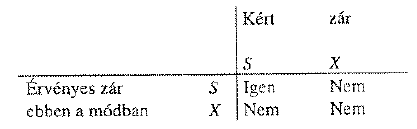
\includegraphics[width=0.5\linewidth]{img/deadlock}
		\caption{Példa holtpontra.}
		\label{fig:deadlock}
	\end{figure}
	
	\paragraph{Különböző zármódú zárolási rendszerek}
	
	\noindent \textbf{Osztott és kizárolagos zárak}: Tetszőleges adatbáziselemet vagy egyszer lehet zárolni kizárólagosan (írásra), vagy
	többször osztottan (olvasásra). Kizárólagosan zárolt elemet nem lehet osztottan zárolni, illetve osztottan zárolt elemet
	nem lehet kizárólagosan zárolni. Ha X-et írni akarjuk, akkor X-re kizárólagos zárral kell rendelkeznünk, ha olvasni, akkor
	elég az osztott is, de kizárólagos zárral is tudjuk olvasni.\\
	
	\noindent \textbf{Kompatibilitási mátrix}: A kompatibilitási mátrix minden egyes zármódhoz rendelkezik egy sorral és egy oszloppal.
	A sorok egy másik tranzakció által az X elemre már érvényes záraknak felelnek meg, az oszlopok pedig az X-re kért zármódoknak
	felelnek meg. A használat szabálya: C módú zárat akkor és csak akkor engedélyezhetünk, ha táblázat minden olyan R sorára, amelyre
	más tranzakció már zárolta X-et R módban, a C oszlopban "Igen" szerepel.
	
	\begin{figure}[H]
		\centering
		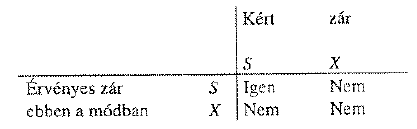
\includegraphics[width=0.5\linewidth]{img/kompmatrix}
		\caption{Osztott és kizárólagos zárak kompatibilitási mátrixa.}
		\label{fig:kompmatrix}
	\end{figure}
	
\end{document}